\providecommand{\main}{../../..}
\documentclass[\main/dresen_thesis.tex]{subfiles}
\renewcommand{\thisPath}{\main/chapters/appendix/additionalExperimentalTechniques}
\begin{document}

\chapter{Laboratory Instruments}
\section{PPMS Evercool II - Vibrating Sample Magnetometry}
\label{app:additionalExperimentalTechniques:vsm}
\begin{figure}[h]
  \centering
  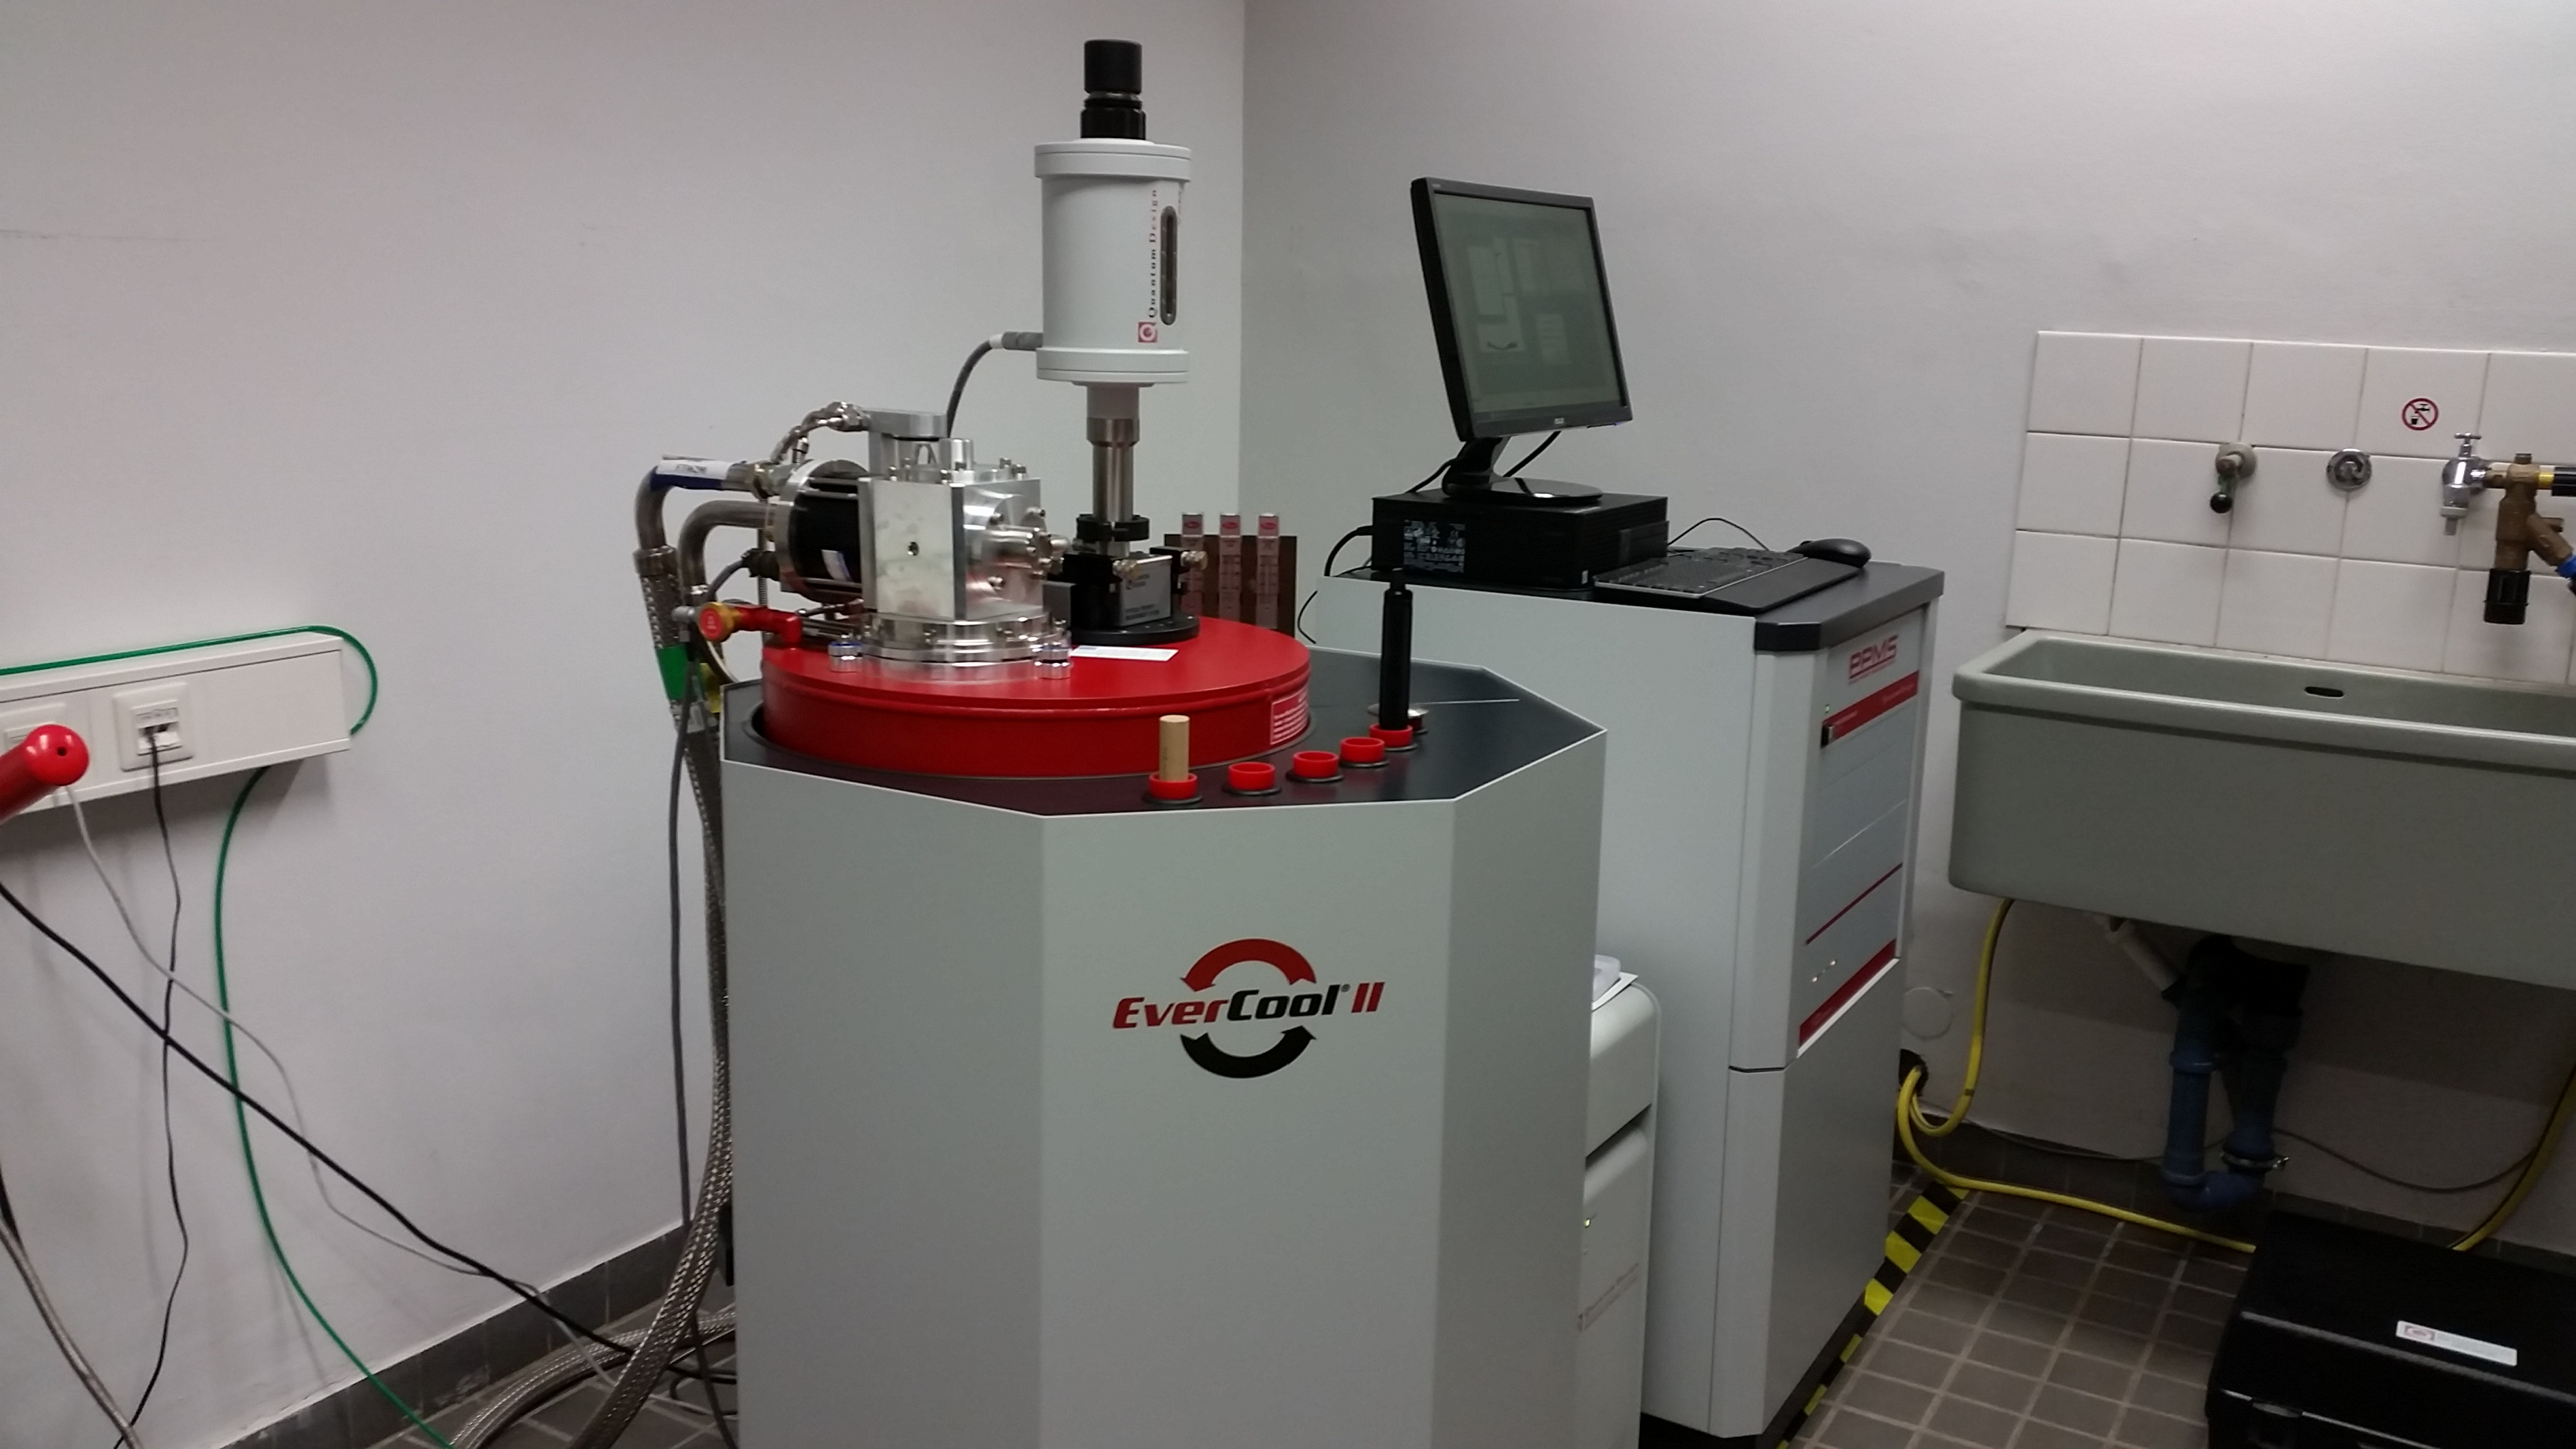
\includegraphics[width=0.7\textwidth]{instruments_ppms}
  \caption{\label{fig:appendix:instruments:ppms}The physical property measurement system (PPMS) Evercool II, which is used to measure the macroscopic magnetization properties by vibrating sample magnetometry.}
\end{figure}

\section{Bruker D8 Advanced - X-Ray Reflectometry}
\label{app:additionalExperimentalTechniques:xrr}
\begin{figure}[h]
  \centering
  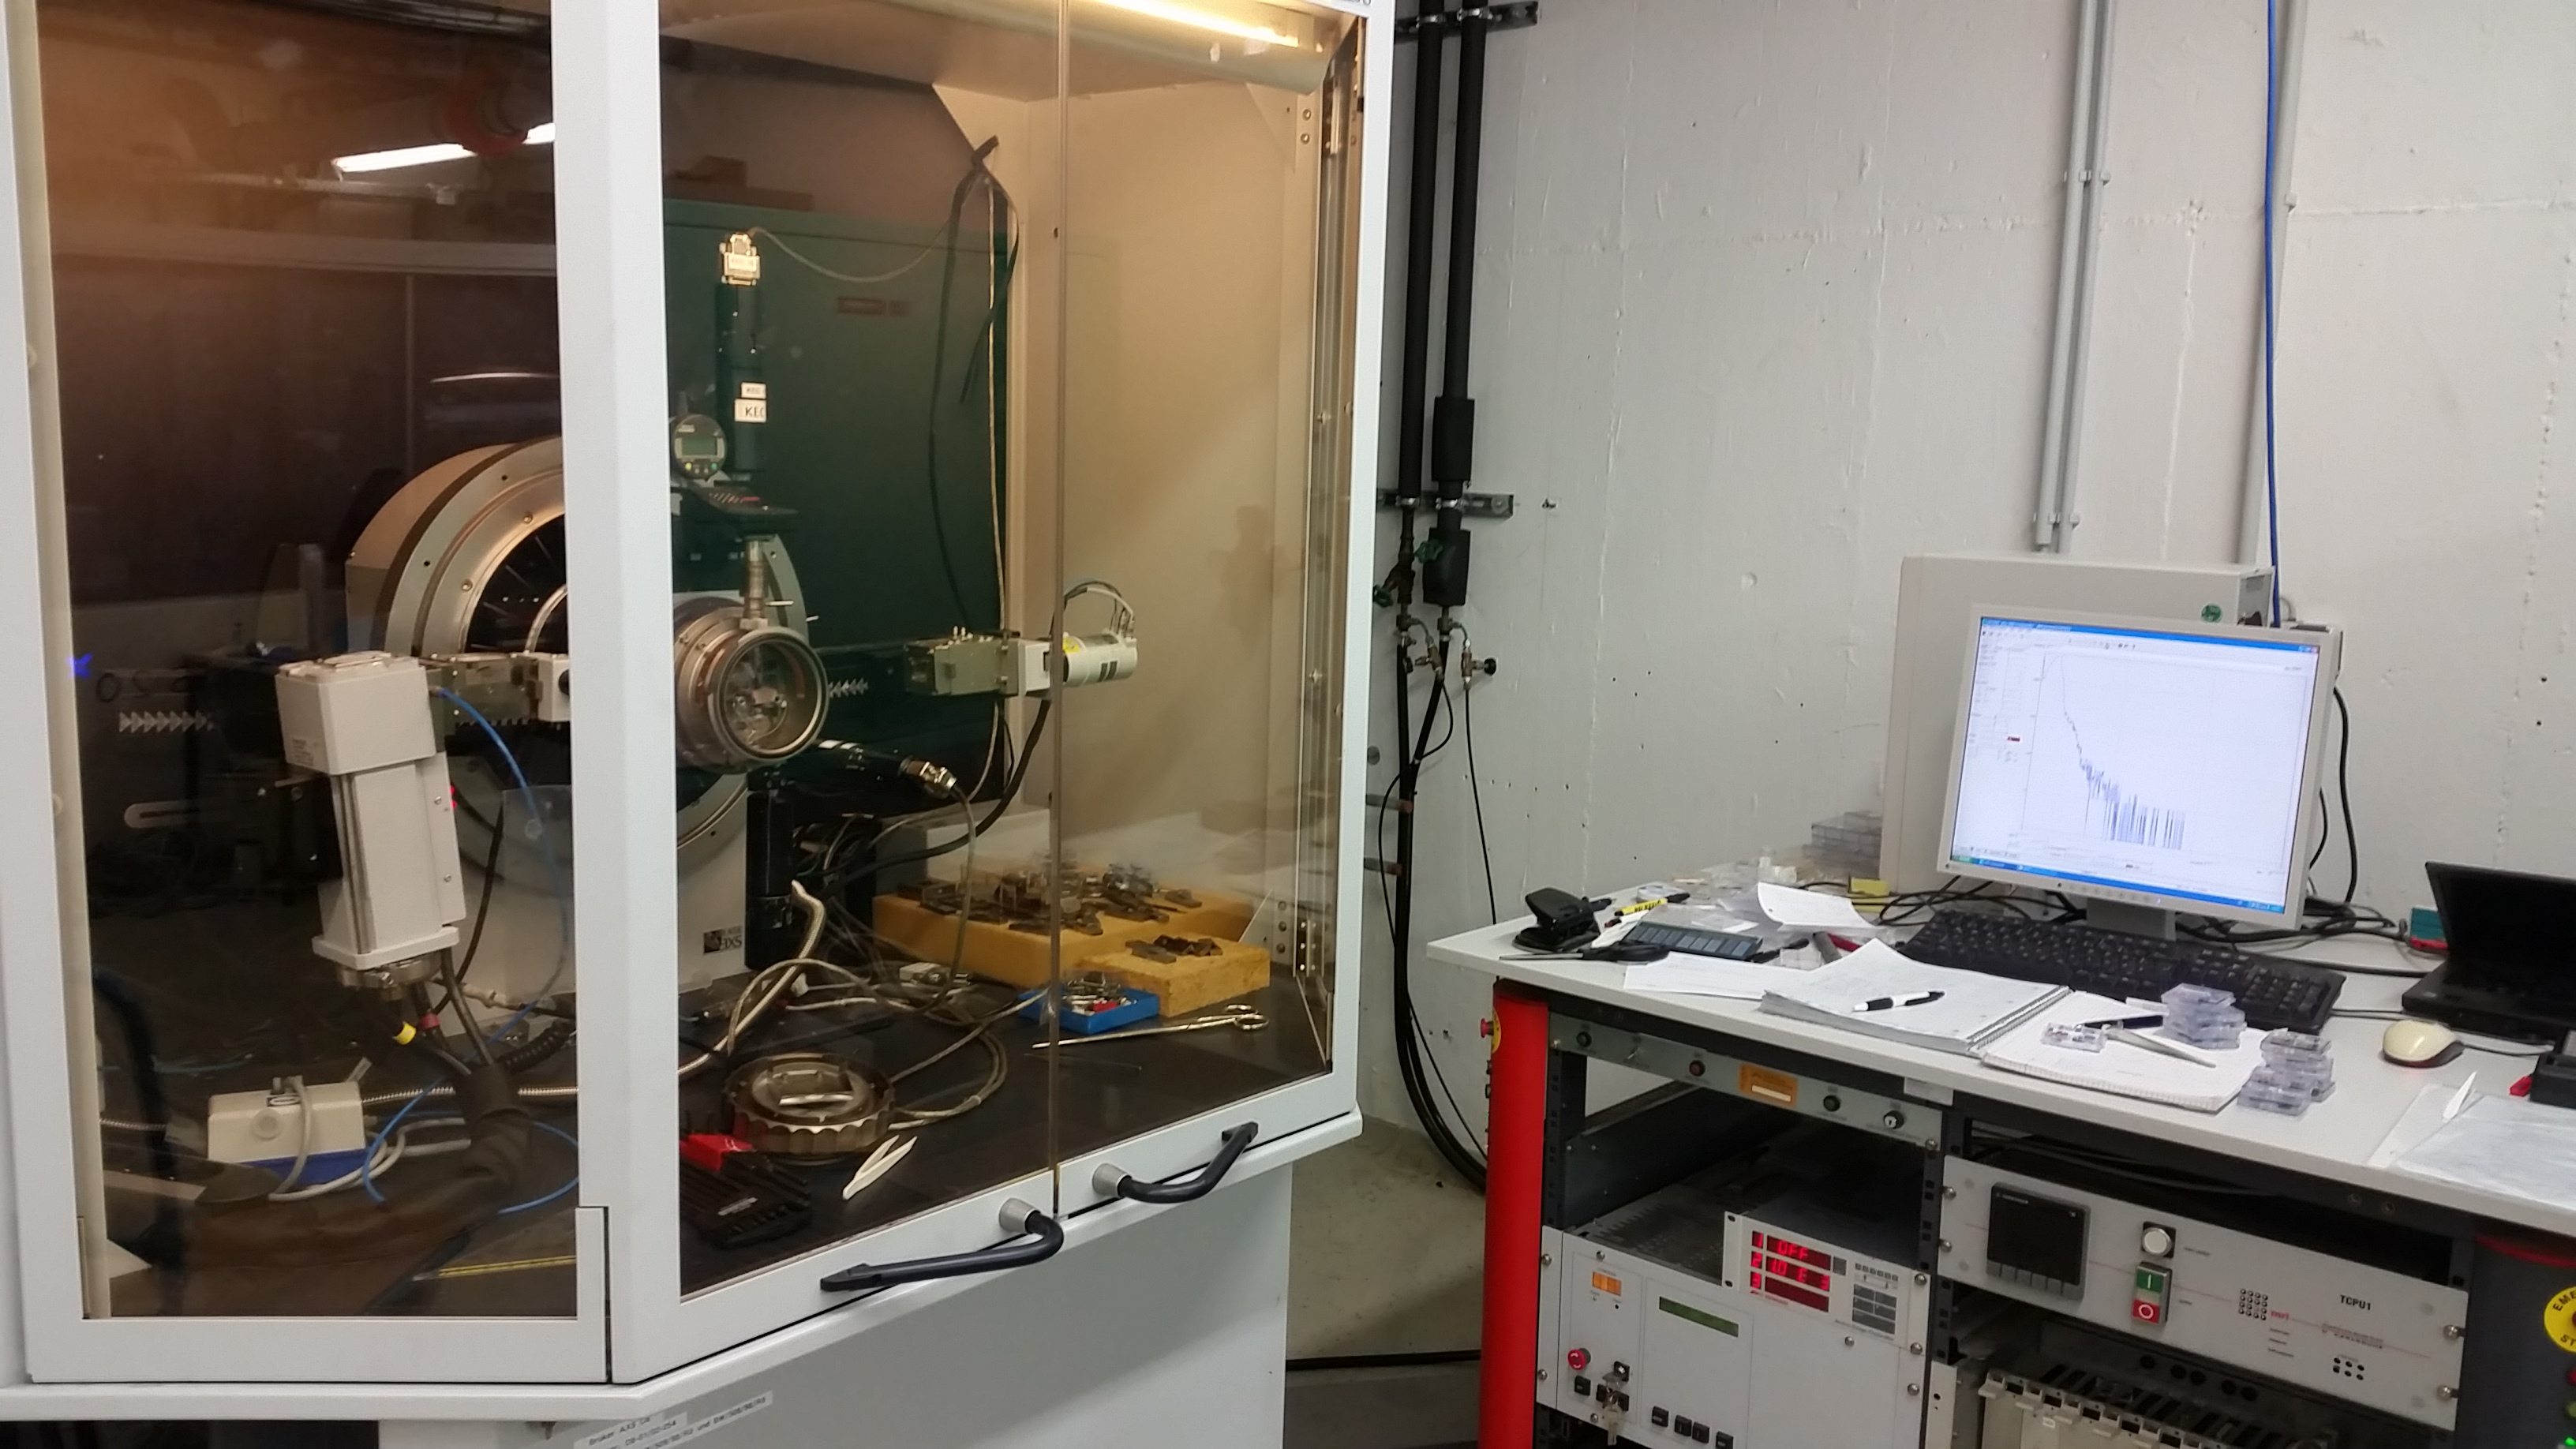
\includegraphics[width=0.7\textwidth]{instruments_brukerD8}
  \caption{\label{fig:appendix:instruments:brukerD8}Bruker D8 instrument, which can be used for x-ray reflectometry and x-ray diffraction.}
\end{figure}
To perform XRR experiments, described in \refapp{app:methods:xrr}, the Bruker D8 instrument in the \textsc{Forchungszentrum J\"ulich} was used.
The Bruker D8 is equipped with a Cu-K$\alpha$ source and a 
For XRR, the incident angle of the beam and the outgoing angle are increased simultaneously to maintain the specular condition while scanning the reflected intensity over $q_z$.
The beam size can be varied by slits and is typically set to $0.2 \unit{mm}$.
To estimate the beam divergence, the direct beam is scanned with the detector in \reffig{fig:appendix:instruments:brukerD8DirectBeam}.
The best fit with a gaussian function results in a divergence of $\Delta \alpha_i \eq 0.01510(4) ^\circ \eq 2.635(7) \cdot 10^{-4}.$
\begin{figure}[h]
  \centering
  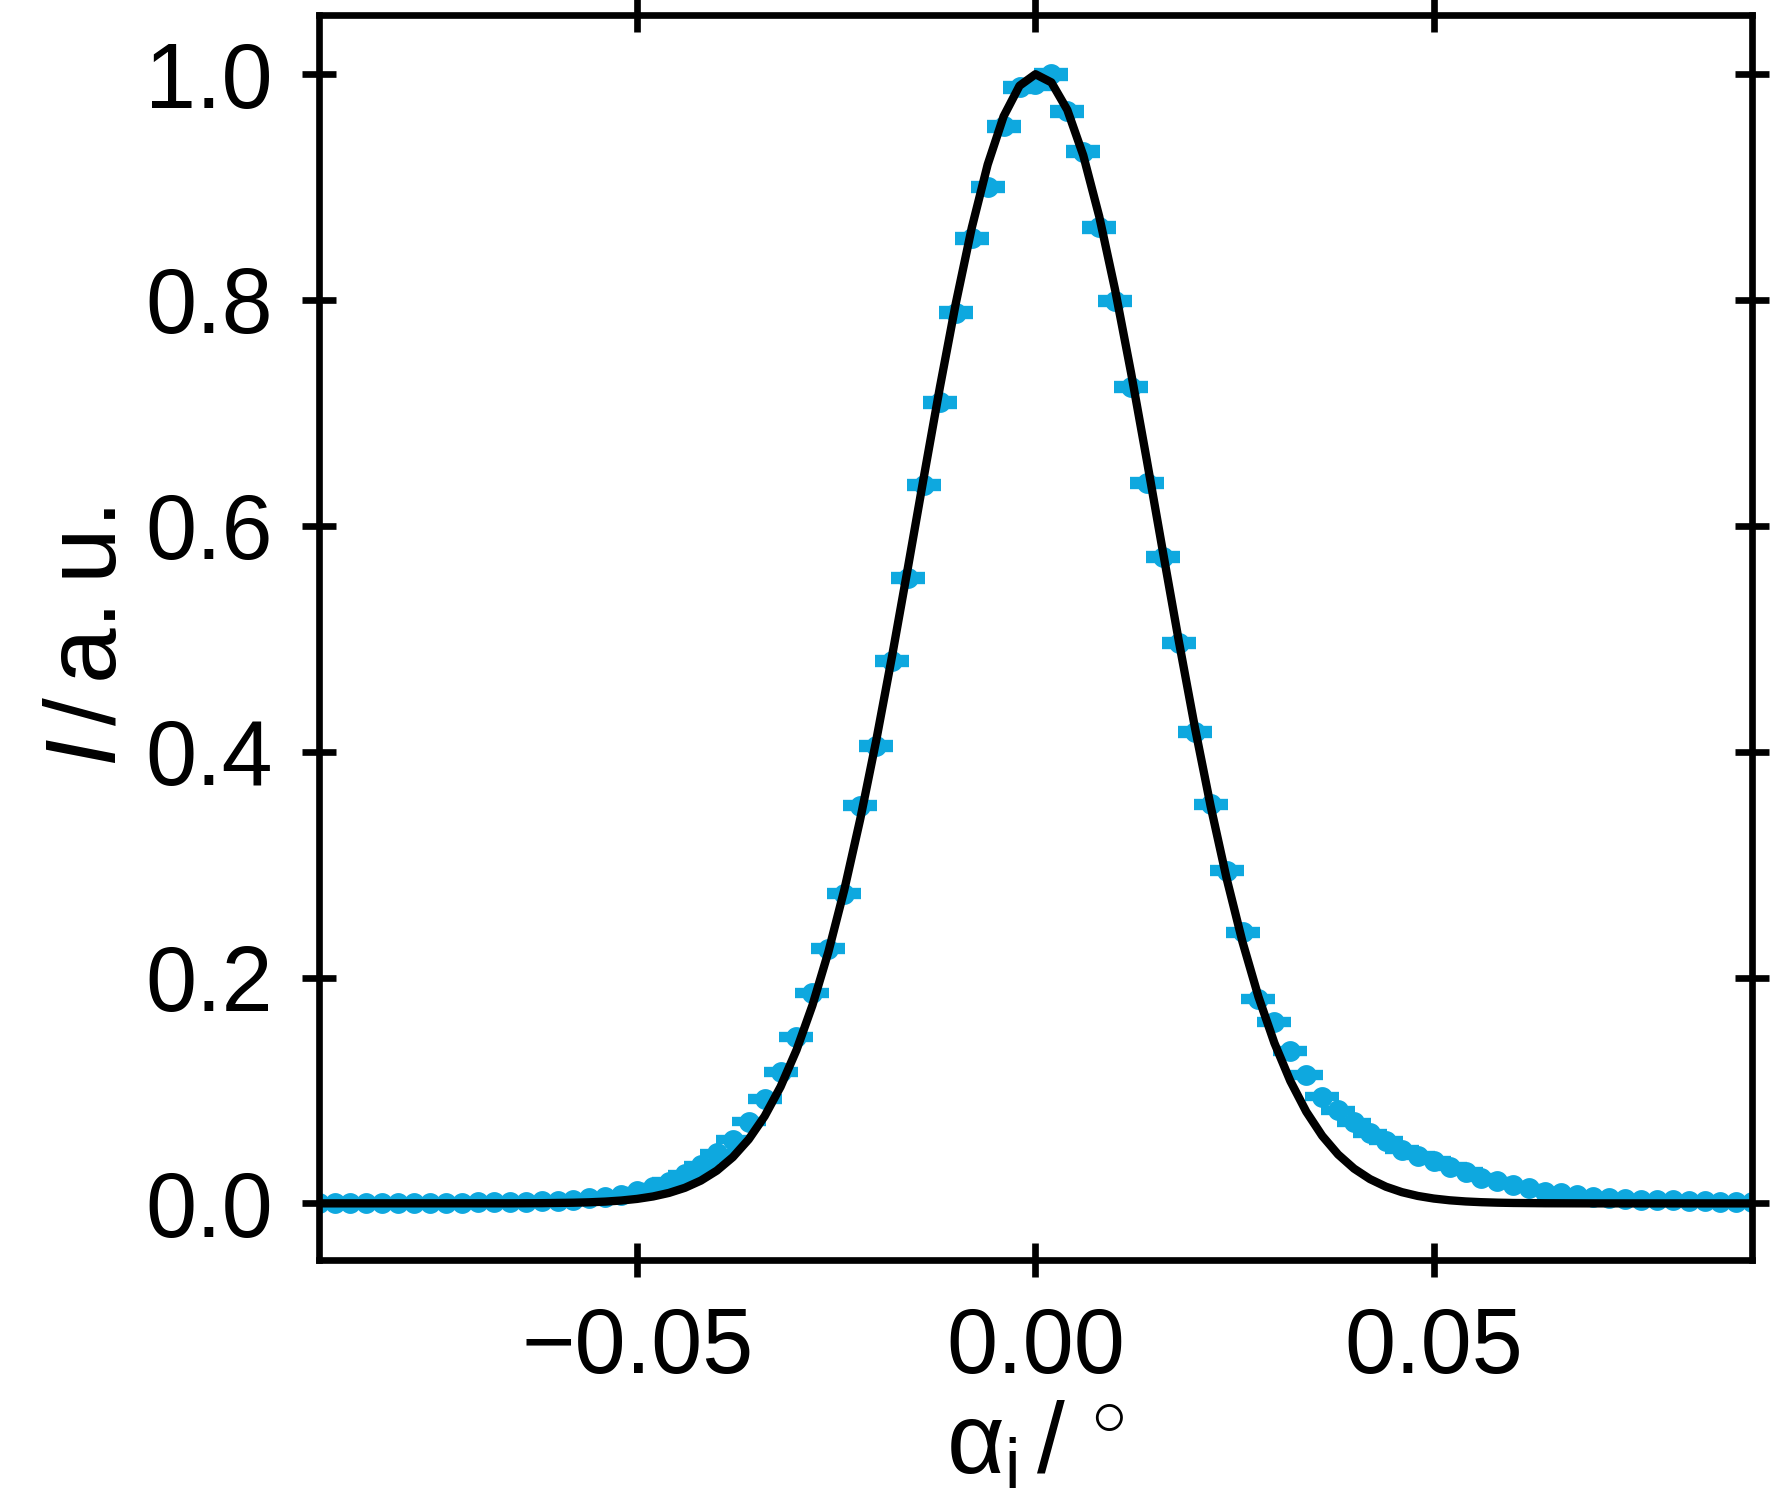
\includegraphics{appendix_instruments_brukerD8DirectBeam}
  \caption{\label{fig:appendix:instruments:brukerD8DirectBeam}Direct beam scan of the Bruker D8 instrument at a beam slit size of $0.2 \unit{mm}$, modelled by a gaussian function to estimate the divergence.}
\end{figure}

\section{X-Ray Diffraction}
\label{app:additionalExperimentalTechniques:xrd}
Daniel Nižňanský from the Department of Inorganic Chemistry at the Charles University in Prague

\section{Neon Zeiss 40 - Scanning Electron Microscopy}
\label{app:additionalExperimentalTechniques:sem}
\begin{figure}[h]
  \centering
  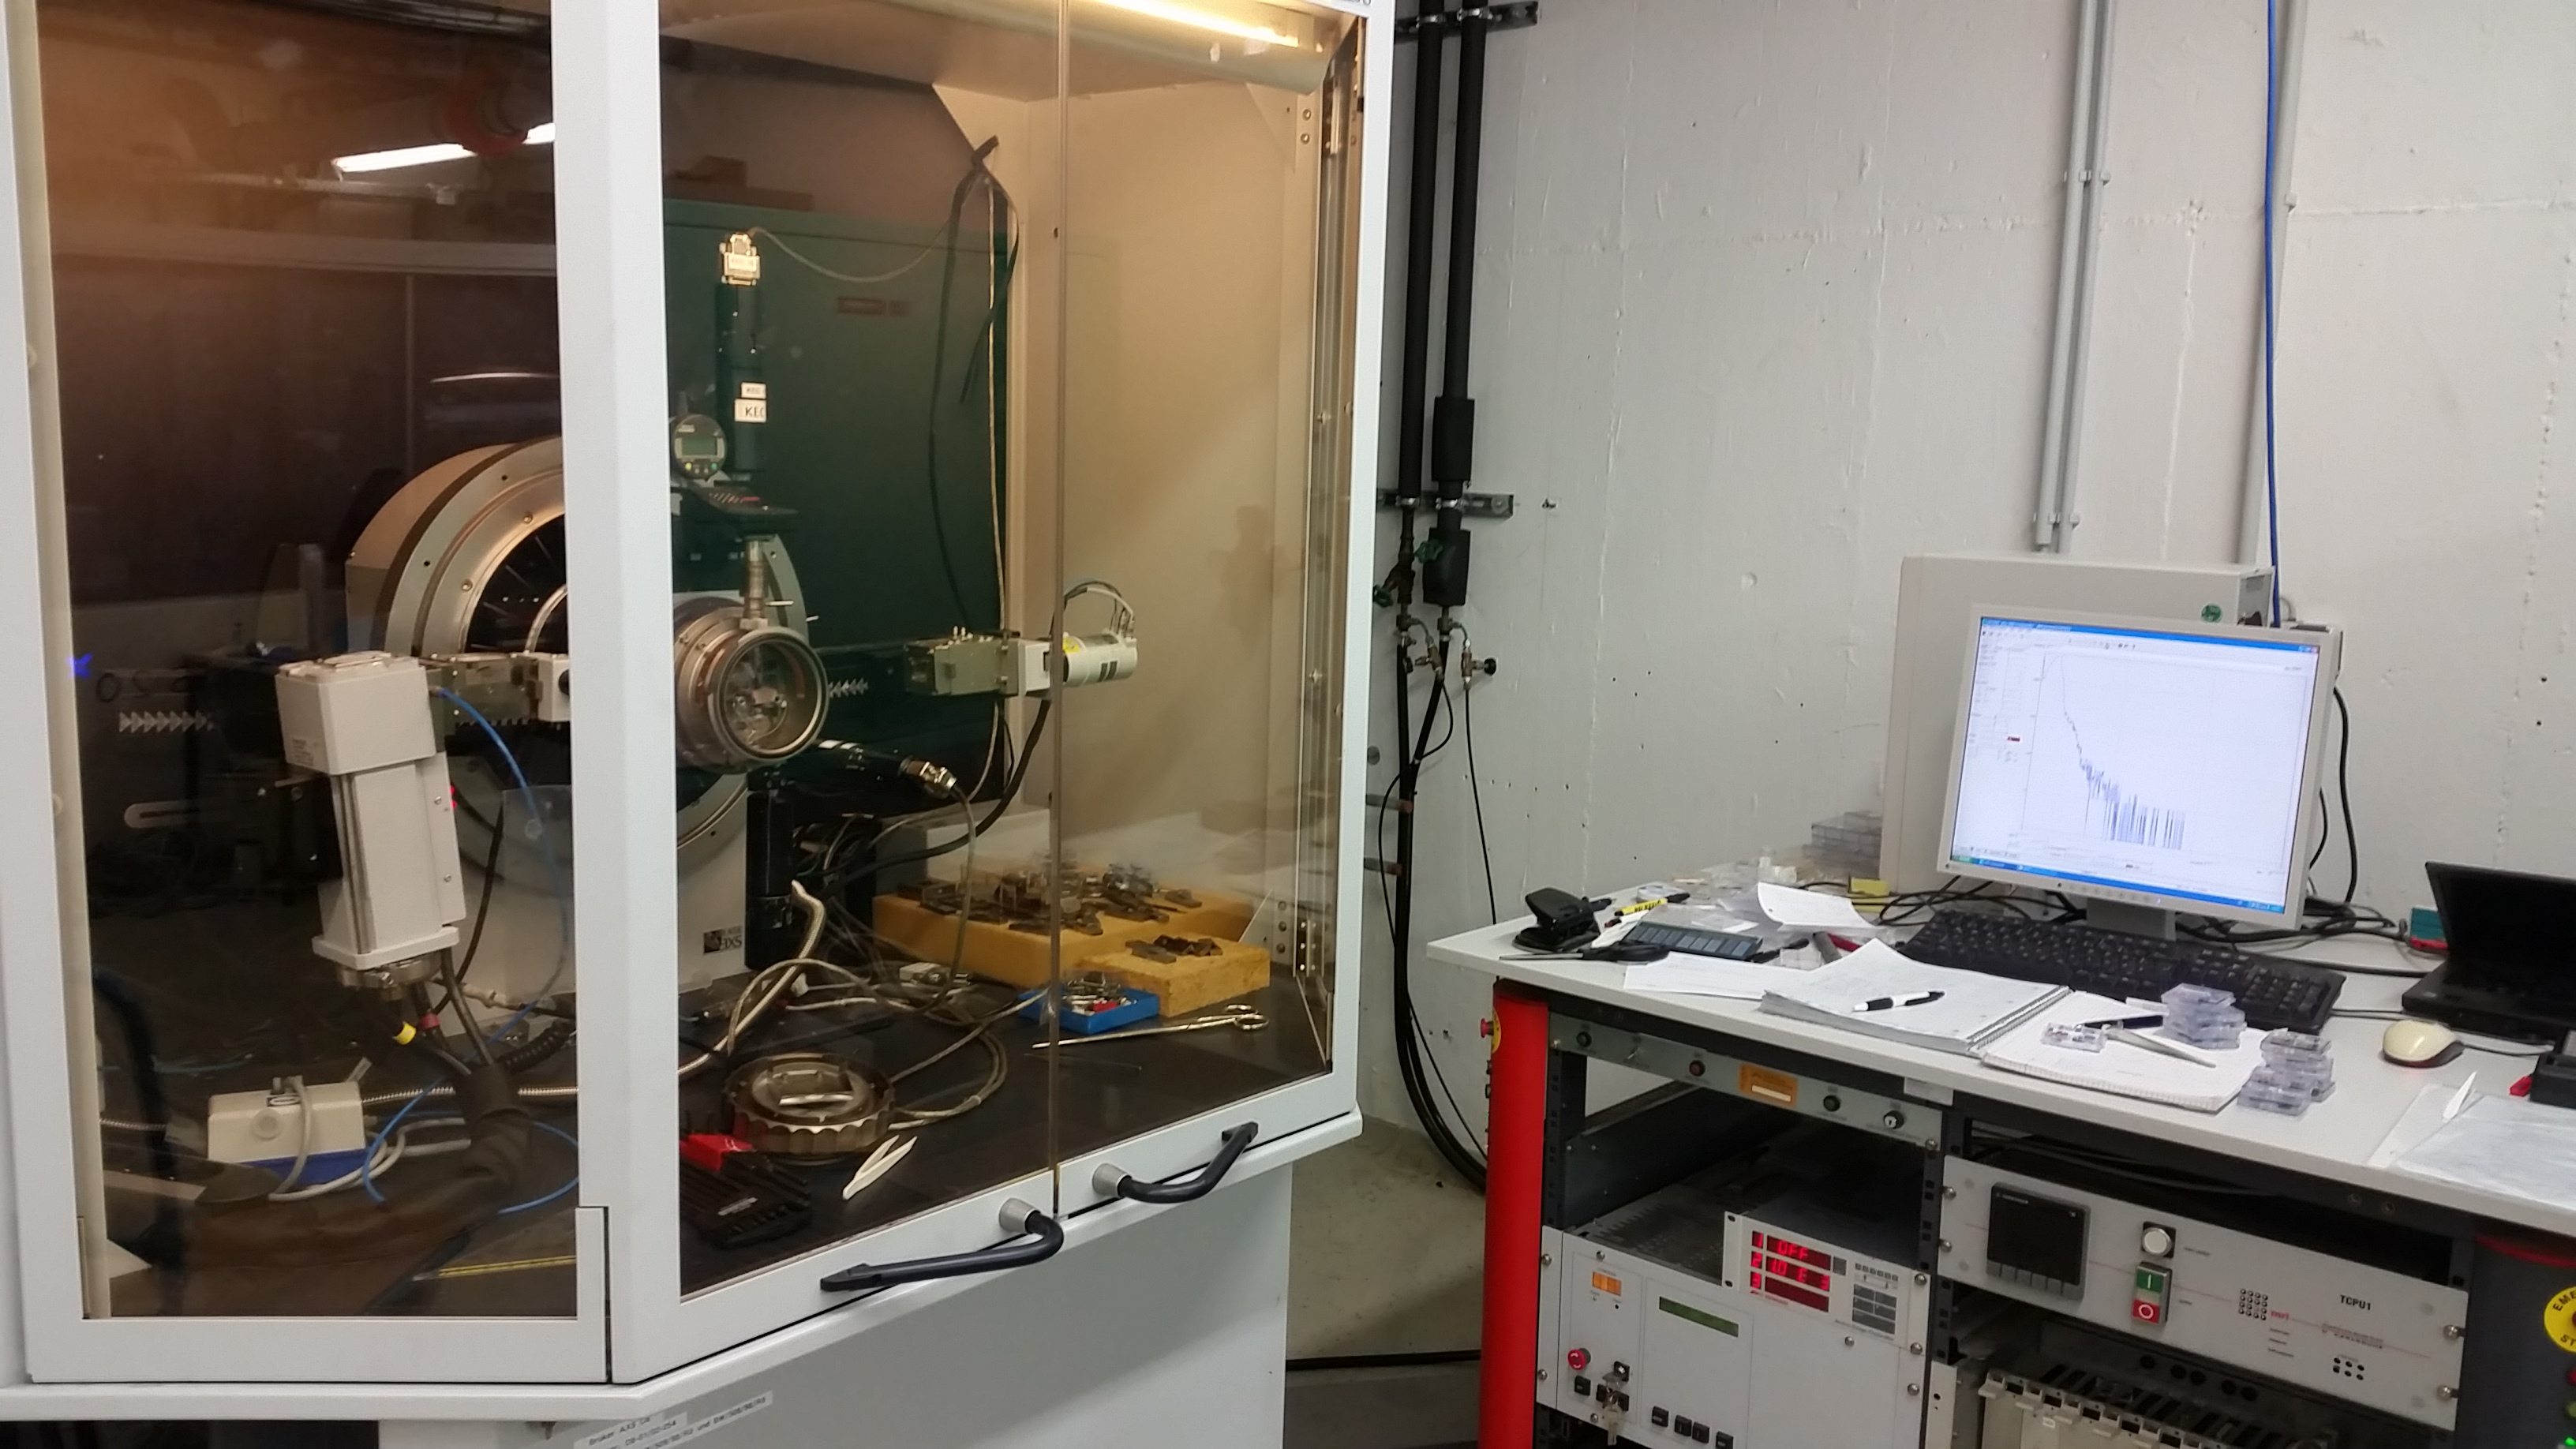
\includegraphics[width=0.7\textwidth]{instruments_brukerD8}
  \caption{\label{fig:appendix:instruments:SEM}Bruker D8 instrument which can be used for x-ray reflectometry and x-ray diffraction.}
\end{figure}

\end{document}
